\documentclass{article}

\usepackage[english]{babel}

% Set page size and margins
\usepackage[a4paper,top=2cm,bottom=2cm,left=3cm,right=3cm,marginparwidth=1.75cm]{geometry}

% Useful packages
\usepackage{amsmath}
\usepackage{graphicx}
\usepackage[colorlinks=true, allcolors=blue]{hyperref}

\title{Real-Time Stress Detection using Wearable Smartwatch \& Machine Learning}
\author{Md Tariqul Islam}
\date{April 24, 2023} % Add your custom date here

\begin{document}
\maketitle
\begin{table}[h]
    \centering
    \begin{tabular}{ll}
        Registration number: & \textcolor{red}{2200862}\\
        Link to GitHub: & \url{https://github.com/tariqeee/CE888/tree/main/CE888%20assignment-2}\\
    \end{tabular}
\end{table}



\begin{table}[h]
    \centering
    \begin{tabular}{lc}
        Executive summary with introduction (max.\ 200 words) & \textcolor{red}{220}\\
        Main findings and Discussion (max.\ 600 words) & \textcolor{red}{689}\\
        Conclusions (max.\ 300 words) & \textcolor{red}{253}\\
        \hline
        Total word count & \textcolor{red}{1,162}\\
    \end{tabular}
    %\caption{Word counts for each section.}
\end{table}

\tableofcontents

\clearpage

\begin{abstract}
Stress, being a subjective experience, varies from one individual to another, causing generic stress prediction models, which aim to predict stress for any person, to underperform. Although individual-specific models that predict stress for a particular person yield more accurate results, they are inflexible and costly to implement in real-life situations. For example, a person-specific stress monitoring system in a workplace would necessitate collecting new data and training new models for every employee. Additionally, due to the ever-changing nature of stress and unforeseen events, models tend to deteriorate over time and demand expensive regular updates \cite{zhang2017}.

This paper introduces a practical, efficient, and cost-effective calibration method that employs physiological data from a large population to create accurate, personalized stress prediction models available on GitHub. Our approach is validated using two stress datasets, demonstrating improved performance in terms of accuracy, F1 score, precision, and support. For example, both models achieved over 80\% accuracy, making them suitable for hospital applications. To further enhance accuracy, more data is needed, and advanced deep learning models equipped with robust prediction and detection tools can be utilized \cite{nkurikiyeyezu}.
\end{abstract}



\textbf{Introduction:} Stress is a pervasive problem in contemporary society, impacting individuals' physical and mental health \cite{cohen2007}. The capability to precisely predict and monitor stress levels has grown increasingly crucial, as it offers essential insights for people to better manage their stress \cite{sharma2012}. This research aims to develop a machine-learning model for stress prediction using physiological indicators such as heart rate and skin conductance \cite{healey2005}. By presenting the main findings, we aspire to illuminate the potential applications of machine learning in stress management \cite{calvo2010} and contribute to the advancement of more effective stress monitoring methodologies \cite{sano2013}.





\section{Main Findings}

\subsection{Dataset Description}
The study makes use of secondary data from GitHub. There is a correlation between the parameters EDAR\_MEAN, EDAR\_STD, NUM\_PEAKSR, HRR\_MEAN, HRR\_STD, TEMPR\_MEAN, TEMPR\_STD, and STRESS, as shown in Ravi, M. S. Stress-detection-in-nurse [8] as shown in Table~\ref{tab:table1} There are 8 columns and 12,445 rows in the dataset. To ensure the accuracy of the data being analyzed, it is essential to verify the datatype of each character during the data preparation process. There is one int64 property (STRESS LEVEL) and seven float64 attributes (EDAR\_MEAN, EDAR\_STD, NUM\_PEAKSR, HRR\_MEAN, HRR\_STD, TEMPR\_MEAN, and TEMPR\_STD) in the dataset, which comprises both int64 and float64 datatypes (Table~\ref{tab:table2} \& Table~\ref{tab:table3}).
\vspace{0.01cm}




\begin{table}[htbp]
  \centering
  \caption{Dataset }
    \label{tab:table1}
  \resizebox{\textwidth}{!}{%
    \begin{tabular}{|l|l|l|l|l|l|l|l|l|}
      \hline
      EDAR\_Mean & EDAR\_Std & Num\_PeaksR & HRR\_Mean & HRR\_Std & TEMPR\_Mean & TEMPR\_Std & Stress \\ \hline
      0.105191   & 0.035656  & 0.0         & 0.641552  & 0.100525 & 0.821491    & 0.120422   & 0.0     \\ \hline
      0.102822   & 0.023788  & 0.0         & 0.642973  & 0.089270 & 0.827471    & 0.105027   & 0.0     \\ \hline
      0.101157   & 0.018717  & 0.0         & 0.643921  & 0.083372 & 0.832395    & 0.099446   & 0.0     \\ \hline
      0.099952   & 0.011283  & 0.0         & 0.645952  & 0.041375 & 0.837759    & 0.089739   & 0.0     \\ \hline
      0.099298   & 0.005735  & 0.0         & 0.646764  & 0.066093 & 0.843123    & 0.095171   & 0.0     \\ \hline
    \end{tabular}
  }
\end{table}
\vspace{0.01cm}


\begin{table}[htbp]
  \centering
  \caption{DataFrame info}
    \label{tab:table2}
  \begin{tabular}{|l|l|l|l|}
    \hline
    Column & Non-Null Count & Dtype & Memory Usage \\ \hline
    EDAR\_Mean & 12445 non-null & float64 & 777.9 KB \\ \hline
    EDAR\_Std & 12445 non-null & float64 & \\ \hline
    Num\_PeaksR & 12445 non-null & float64 & \\ \hline
    HRR\_Mean & 12445 non-null & float64 & \\ \hline
    HRR\_Std & 12445 non-null & float64 & \\ \hline
    TEMPR\_Mean & 12445 non-null & float64 & \\ \hline
    TEMPR\_Std & 12445 non-null & float64 & \\ \hline
    Stress & 12445 non-null & float64 & \\ \hline
  \end{tabular}
\end{table}
\newpage



\begin{table}[htbp]
  \centering
  \caption{Descriptive statistics}
    \label{tab:table3}
  \resizebox{\textwidth}{!}{%
  \begin{tabular}{|l|r|r|r|r|r|r|r|r|}
    \hline
    & count & mean & std & min & 25\% & 50\% & 75\% & max \\ \hline
    EDAR\_Mean & 12445.0 & 0.209896 & 0.104536 & 0.0 & 0.143117 & 0.206731 & 0.259721 & 1.0 \\ \hline
    EDAR\_Std & 12445.0 & 0.063885 & 0.082410 & 0.0 & 0.019800 & 0.039781 & 0.075773 & 1.0 \\ \hline
    Num\_PeaksR & 12445.0 & 0.074126 & 0.181042 & 0.0 & 0.000000 & 0.000000 & 0.000000 & 1.0 \\ \hline
    HRR\_Mean & 12445.0 & 0.531330 & 0.236169 & 0.0 & 0.328595 & 0.573044 & 0.740726 & 1.0 \\ \hline
    HRR\_Std & 12445.0 & 0.058898 & 0.030202 & 0.0 & 0.043969 & 0.054869 & 0.068181 & 1.0 \\ \hline
    TEMPR\_Mean & 12445.0 & 0.467482 & 0.206970 & 0.0 & 0.322371 & 0.512487 & 0.625923 & 1.0 \\ \hline
    TEMPR\_Std & 12445.0 & 0.082092 & 0.047557 & 0.0 & 0.056860 & 0.072770 & 0.093023 & 1.0 \\ \hline
    Stress & 12445.0 & 0.949779 & 0.903741 & 0.0 & 0.000000 & 1.000000 & 2.000000 & 2.0 \\ \hline
  \end{tabular}%
  }
\end{table}



\subsection{Data Cleaning}
Examining the raw data to find any problems that need to be fixed is known as data cleaning Table~\ref{tab:table4}. Erroneous data, inconsistent datasets, and incomplete data are to be eliminated. In this dataset, there are no attributes with missing values. 



\begin{table}[htbp]
  \centering
  \caption{DataFrame with zero null values}
  \label{tab:table4}
  \begin{tabular}{|l|l|}
    \hline
    Column & Null Values Count \\ \hline
    EDAR\_Mean & 0 \\ \hline
    EDAR\_Std & 0 \\ \hline
    Num\_PeaksR & 0 \\ \hline
    HRR\_Mean & 0 \\ \hline
    HRR\_Std & 0 \\ \hline
    TEMPR\_Mean & 0 \\ \hline
    TEMPR\_Std & 0 \\ \hline
    Stress & 0 \\ \hline
  \end{tabular}
\end{table}



A color palette Figure~\ref{fig:figure5} shows the distinctive hues used in the visualizations. Following a breakdown of the data by stress level, mean and standard deviation are used as an aggregate Table~\ref{tab:table5}. Indicators of stress levels are 0 for low, 1 for medium, and 2 for extreme. To determine the relationship between low, medium, and high-stress levels and all other characteristics, a correlation analysis is carried out.

\begin{figure}[htbp]
  \centering
  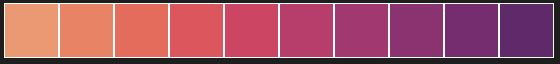
\includegraphics{figure5.jpg}
  \caption{Color Palette Selection for Enhanced Data Visualization}
  \label{fig:figure5}
\end{figure}

\begin{table}[htbp]
\centering
\caption{Sort by Group}
\resizebox{\textwidth}{!}{%
\begin{tabular}{l|rr|rr|rr|rr|rr|rr|rr}
\hline
   & \multicolumn{2}{c|}{EDAR\_Mean} & \multicolumn{2}{c|}{EDAR\_Std} & \multicolumn{2}{c|}{Num\_PeaksR} & \multicolumn{2}{c|}{HRR\_Mean} & \multicolumn{2}{c|}{HRR\_Std} & \multicolumn{2}{c|}{TEMPR\_Mean} & \multicolumn{2}{c}{TEMPR\_Std} \\
Stress & mean & std & mean & std & mean & std & mean & std & mean & std & mean & std & mean & std \\
\hline
0.0 & 0.172351 & 0.104366 & 0.055162 & 0.065891 & 0.070518 & 0.175894 & 0.537097 & 0.243840 & 0.057534 & 0.031945 & 0.541063 & 0.189222 & 0.082361 & 0.051351 \\
1.0 & 0.229339 & 0.099549 & 0.074894 & 0.100680 & 0.078889 & 0.188306 & 0.544647 & 0.206367 & 0.060759 & 0.035588 & 0.391931 & 0.203591 & 0.084292 & 0.043802 \\
2.0 & 0.243203 & 0.092572 & 0.068570 & 0.088467 & 0.075967 & 0.183242 & 0.518548 & 0.239898 & 0.059565 & 0.024887 & 0.419816 & 0.200942 & 0.080754 & 0.044670 \\
\hline
\end{tabular}}
\label{tab:table5}
\end{table}



\subsection{Data Visualization and Exploration }
To make it easier to examine the dataset and understand its structure, data visualization and exploration make the dataset variables visible using histograms (Figure~\ref{fig:figure7}), pair plots, and boxplots. The characteristics EDAR\_MEAN, EDAR\_STD, NUM\_PEAKSR, HRR\_MEAN, HRR\_STD, TEMPR\_MEAN, TEMPR\_STD, and STRESS are shown in a histogram (Figure~\ref{fig:figure8}).

\begin{figure}[htbp]
  \centering
  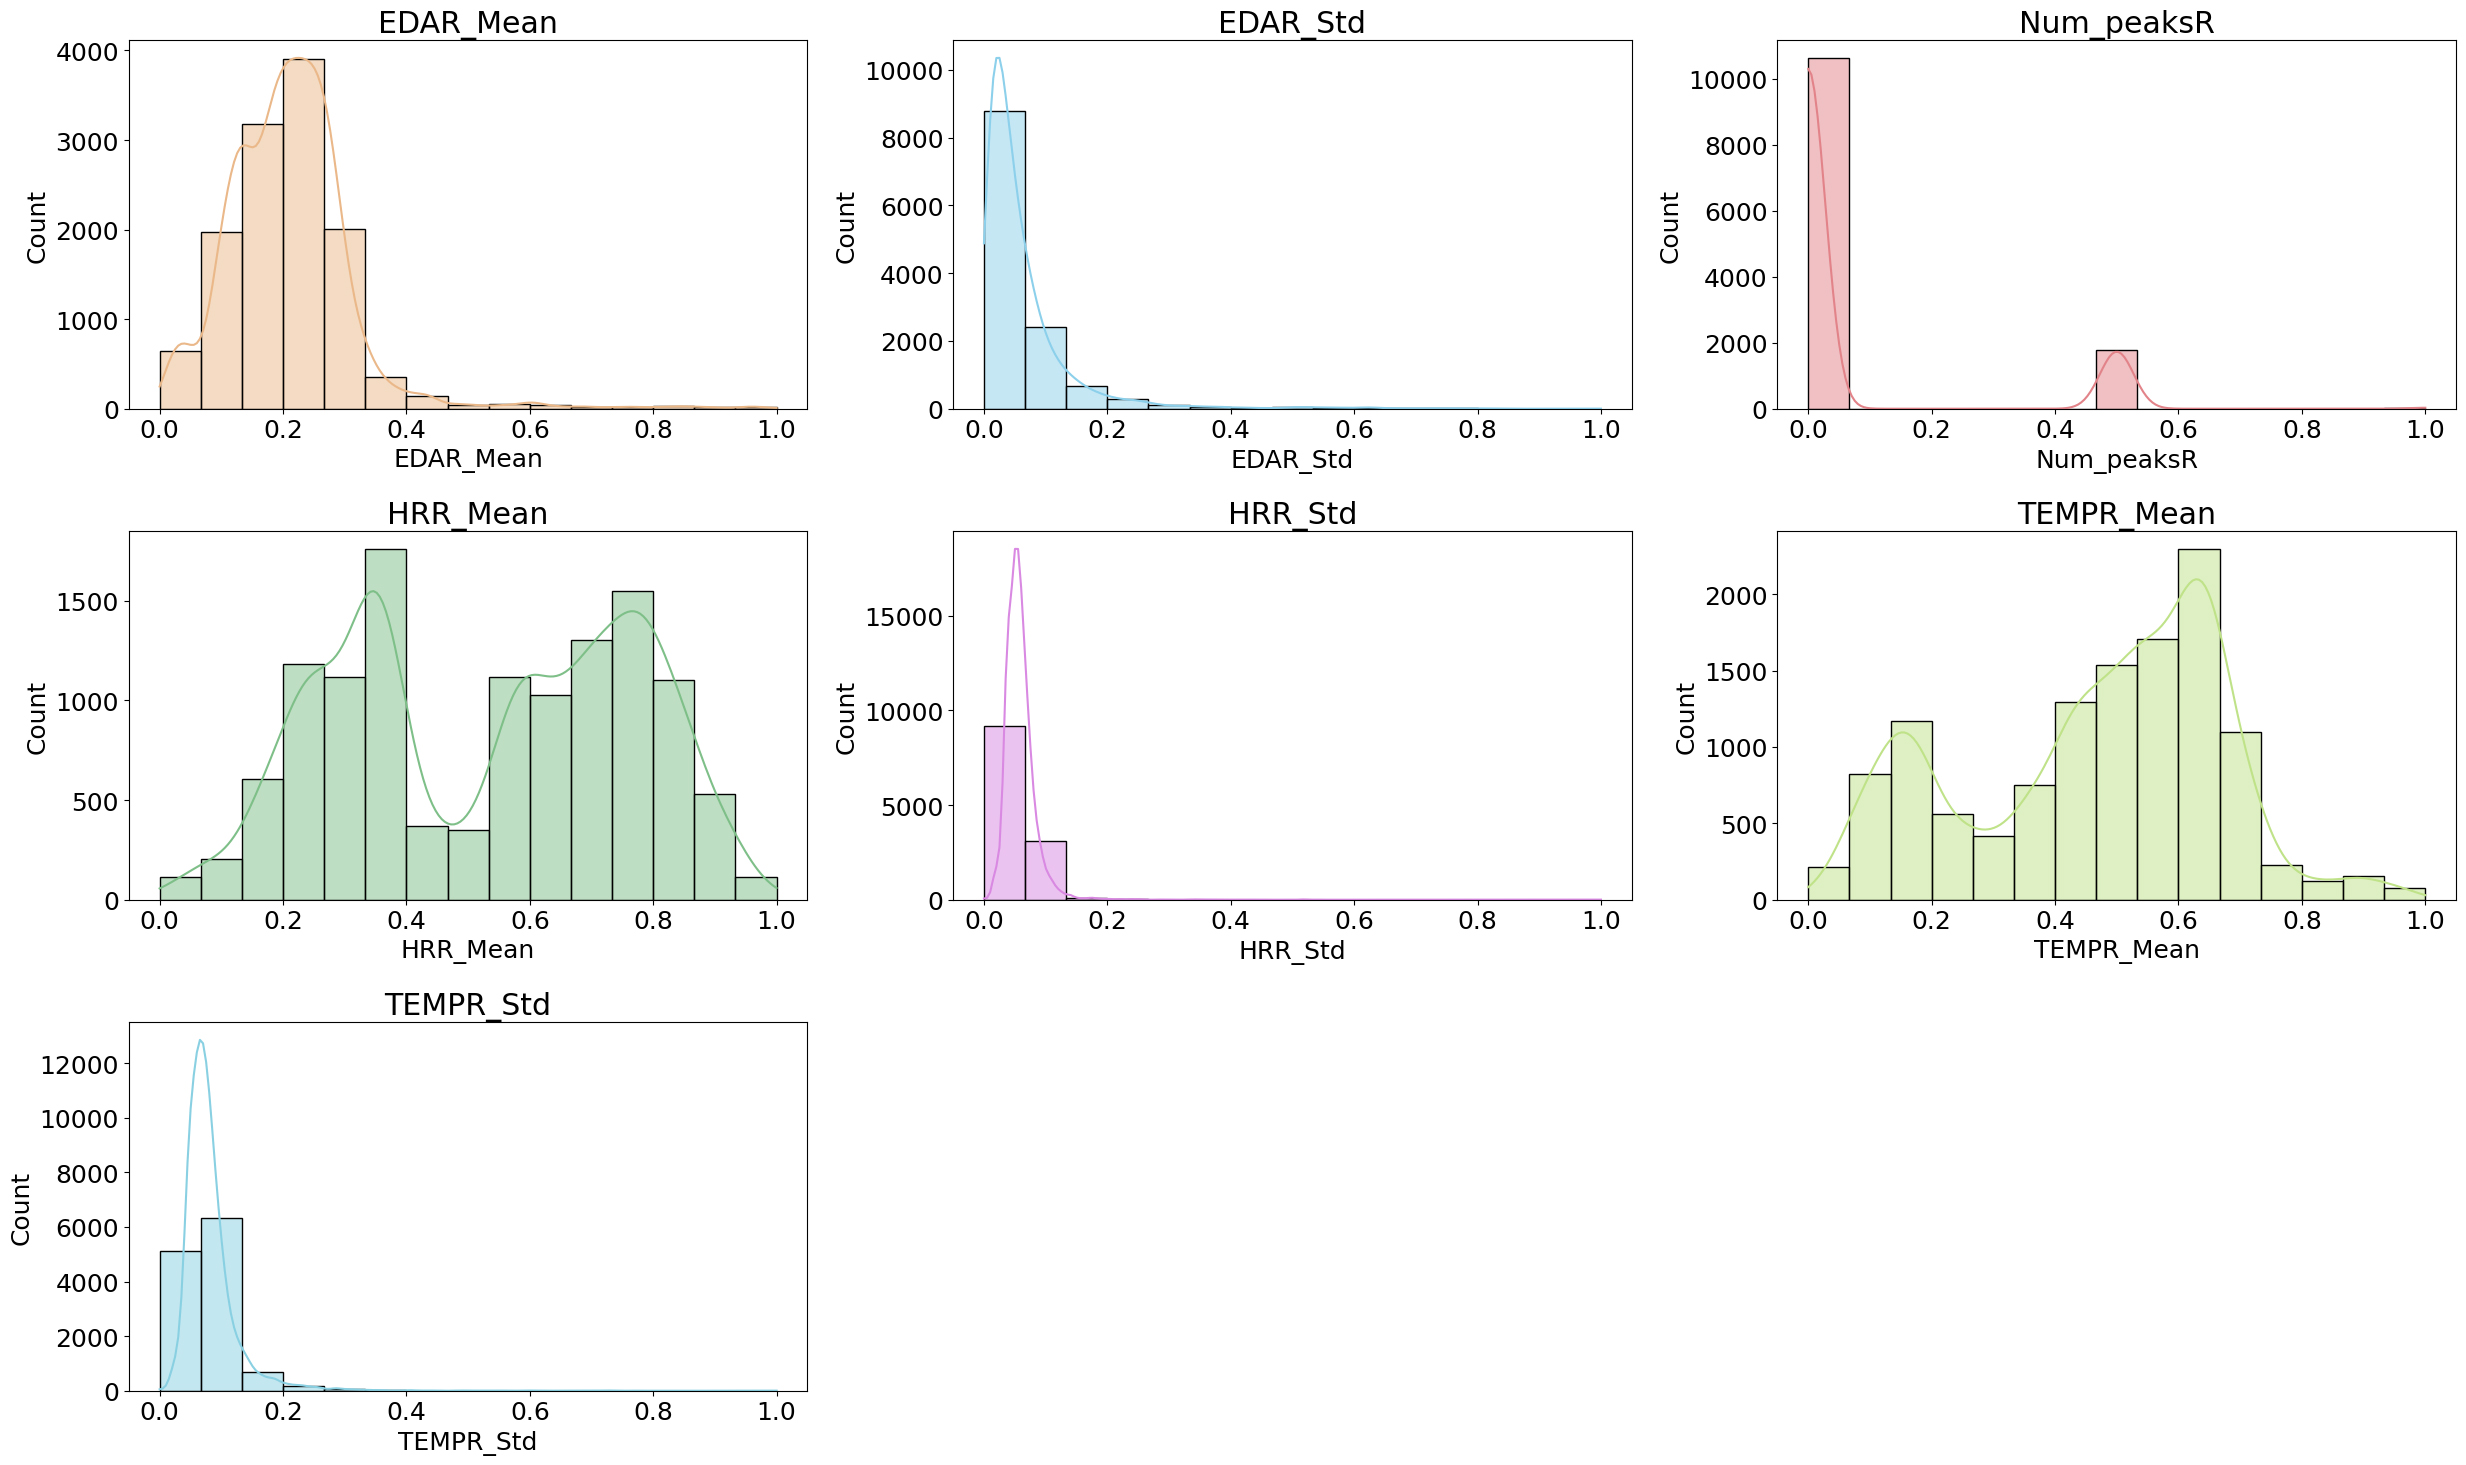
\includegraphics[width=0.8\textwidth]{figure7.jpg}
    \caption{Bar Graph Comparing Stress Levels Across Different Physiological Features}
  \label{fig:figure7}
\end{figure}









\begin{figure}[htbp]
    \centering
    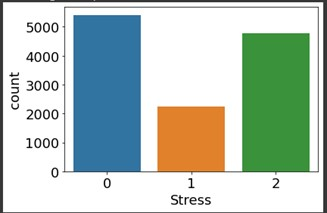
\includegraphics[width=0.6\textwidth]{figure8.jpg}
    \caption{Histogram of Physiological Feature Distributions for Stress Level Assessment}
  \label{fig:figure8}
\end{figure}


Another histogram Figure~\ref{fig:figure8} displays the number of persons in relation to their degree of stress, showing that a low number of people are stressed, followed by a high number, and then a medium level. The value is plotted against several variables using a boxplot Figure~\ref{fig:figure7}, which indicates that the HRR\_STD and TEMPR\_STD have stronger discriminating power and exhibit anomalies, respectively.




\subsection{Correlation}
The next step is to generate a correlation matrix for all the variables in Figure~\ref{fig:figure19}, which demonstrates that the dependent attribute Figure~\ref{fig:figure10}, or stress level, and all the qualities are positively connected Table~\ref{tab:correlation_matrix}.

\begin{figure}[htbp]
    \centering
    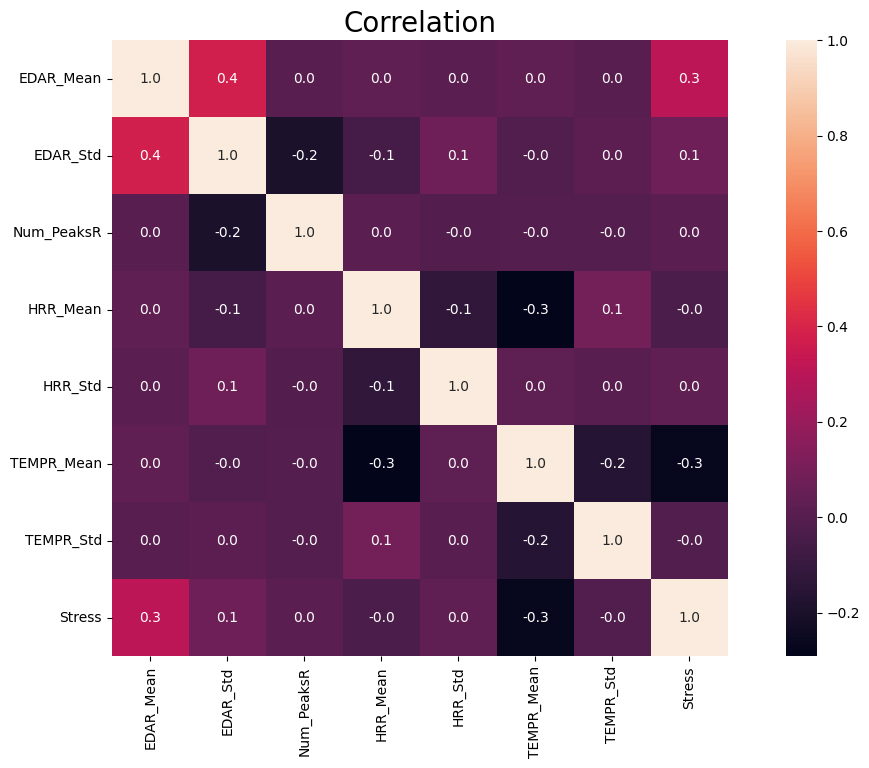
\includegraphics[width=0.8\textwidth]{figure9.jpg}
    \caption{Heatmap of Correlations Between Physiological Features and Stress Levels}
    \label{fig:figure19}
\end{figure}


\begin{figure}[htbp]
    \centering
    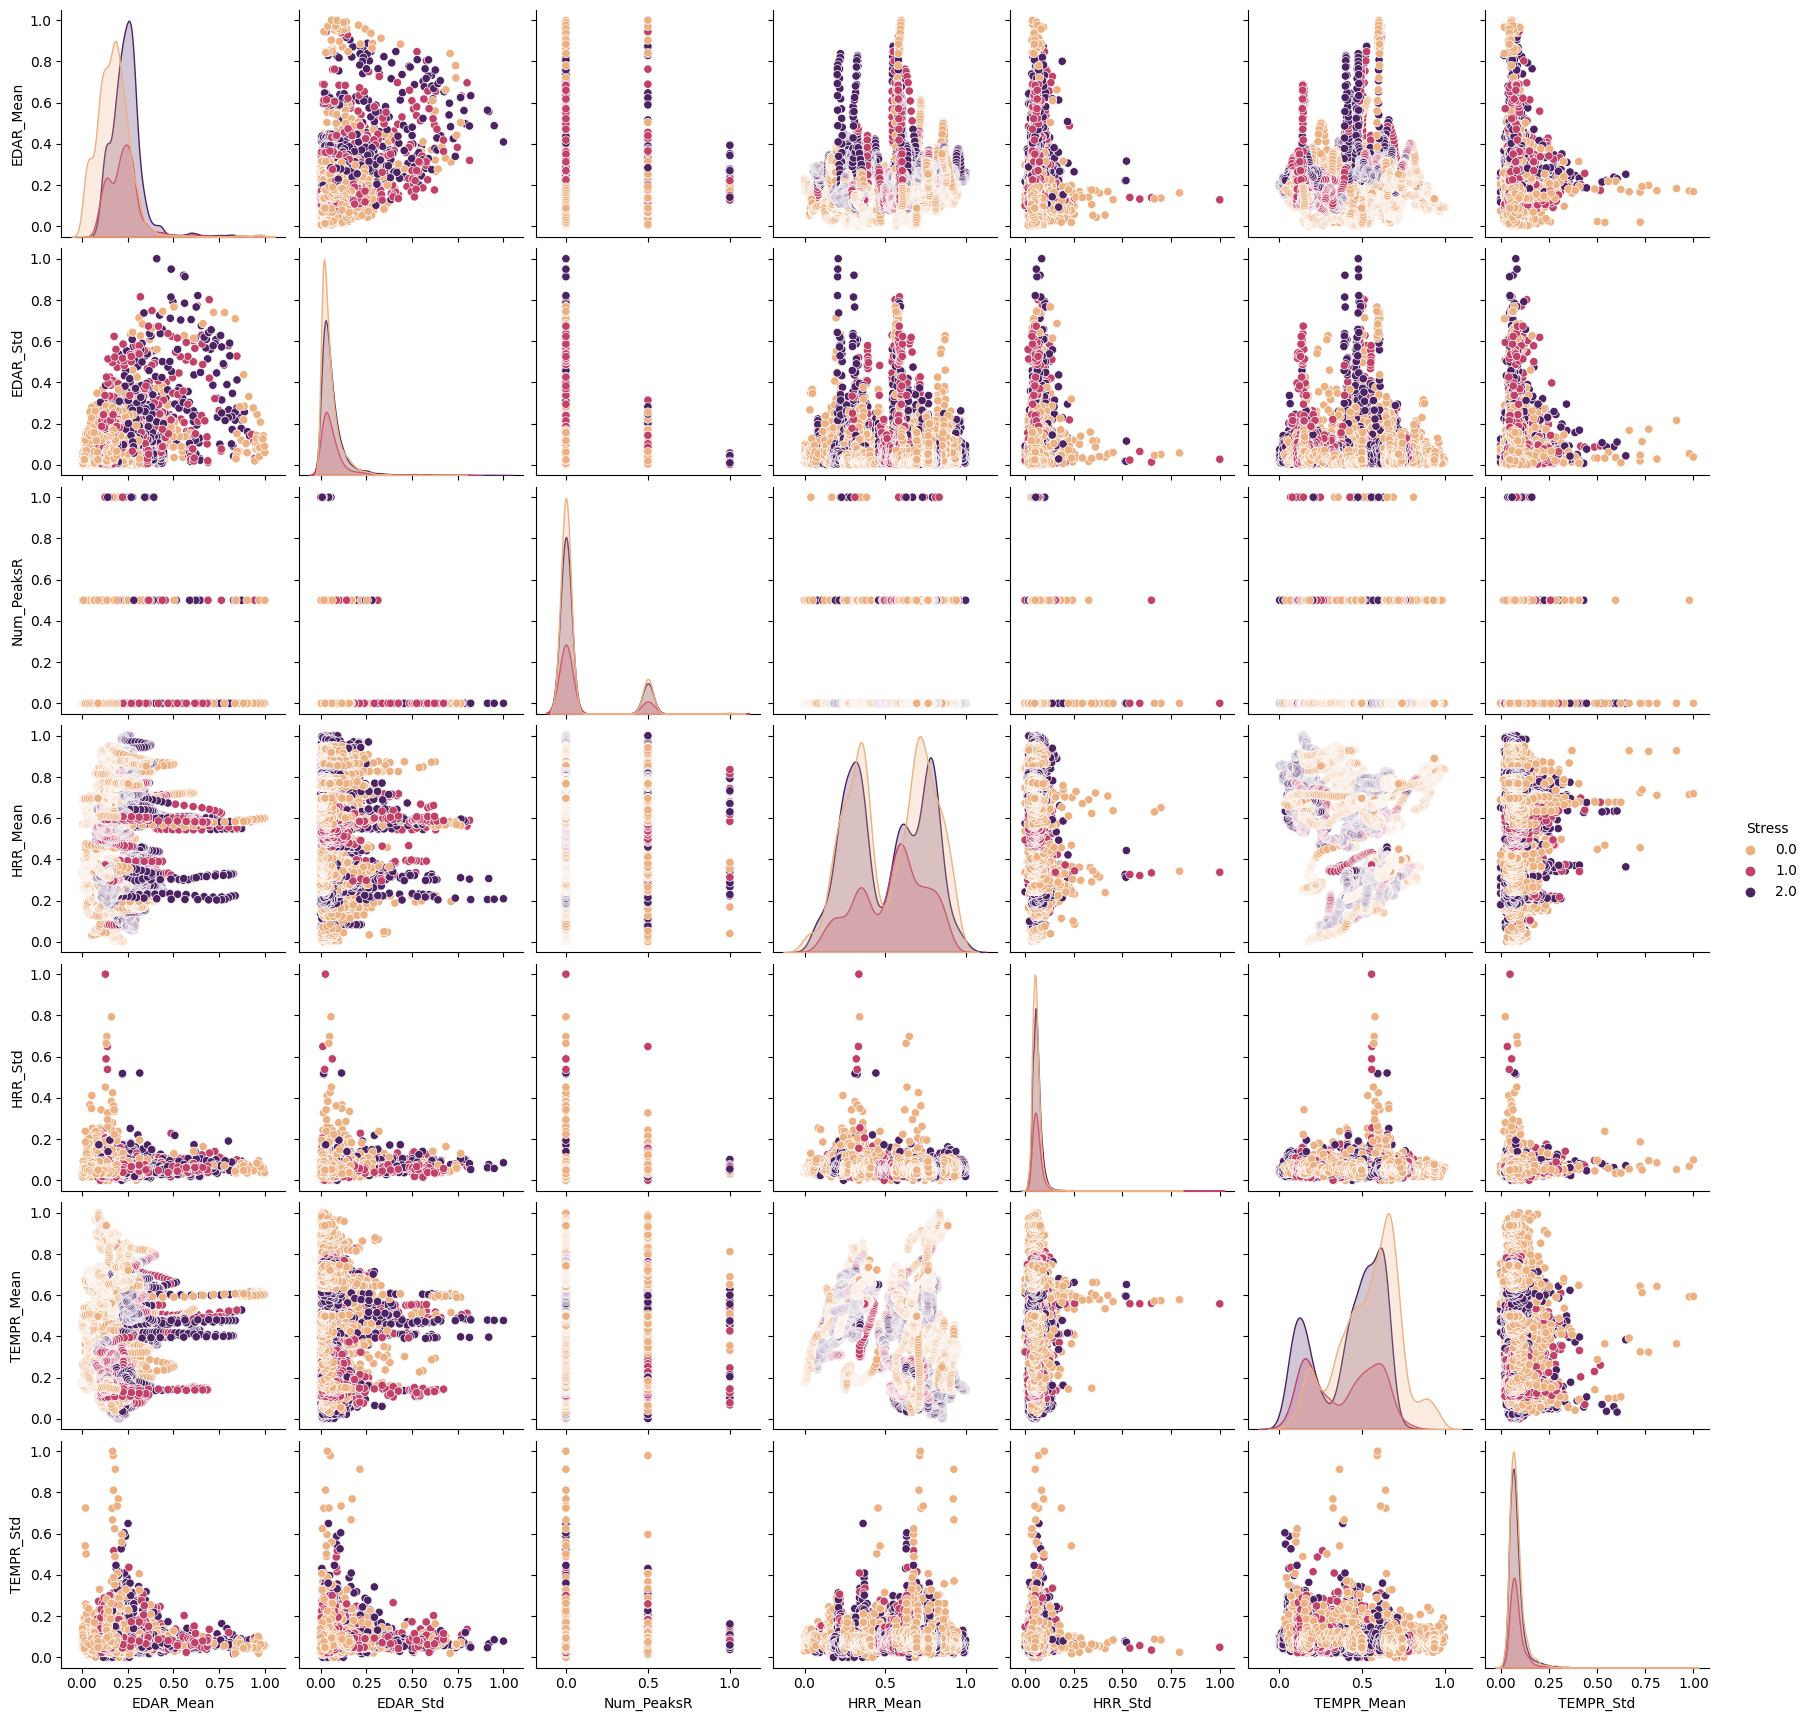
\includegraphics[width=0.8\textwidth]{figure10.jpg}
    \caption{Pair Plot of Physiological Features for Stress Level Analysis}
    \label{fig:figure10}
\end{figure}



\begin{table}[htbp]
    \centering
    \caption{Correlation matrix of all variables}
    \label{tab:correlation_matrix}
    \resizebox{\textwidth}{!}{
        \begin{tabular}{l|rrrrrrrr}
                  & \multicolumn{1}{c}{EDAR\_Mean} & \multicolumn{1}{c}{EDAR\_Std} & \multicolumn{1}{c}{Num\_PeaksR} & \multicolumn{1}{c}{HRR\_Mean} & \multicolumn{1}{c}{HRR\_Std} & \multicolumn{1}{c}{TEMPR\_Mean} & \multicolumn{1}{c}{TEMPR\_Std} & \multicolumn{1}{c}{Stress} \\
        \hline
        EDAR\_Mean   & 1.000000  & 0.375326  & 0.007842  & 0.028150  & 0.012492  & 0.029463  & 0.002551  & 0.308340 \\
        EDAR\_Std    & 0.375326  & 1.000000  & -0.200031 & -0.058697 & 0.073785  & -0.016977 & 0.019933  & 0.075108 \\
        Num\_PeaksR  & 0.007842  & -0.200031 & 1.000000  & 0.013078  & -0.013462 & -0.006776 & -0.005626 & 0.013914 \\
        HRR\_Mean    & 0.028150  & -0.058697 & 0.013078  & 1.000000  & -0.128394 & -0.291501 & 0.090610  & -0.034776 \\
        HRR\_Std     & 0.012492  & 0.073785  & -0.013462 & -0.128394 & 1.000000  & 0.022783  & 0.008214  & 0.031129 \\
        TEMPR\_Mean  & 0.029463  & -0.016977 & -0.006776 & -0.291501 & 0.022783  & 1.000000  & -0.161525 & -0.269011 \\
        TEMPR\_Std   & 0.002551  & 0.019933  & -0.005626 & 0.090610  & 0.008214  & -0.161525 & 1.000000  & -0.014696 \\
        Stress       & 0.308340  & 0.075108  & 0.013914  & -0.034776 & 0.031129  & -0.269011 & -0.014696 & 1.000000
        \end{tabular}
    }
\end{table}

%%%%%%%%%%%%%%%%%%%%%%%%%%%%%%%%%%%%%%%%%%%%%
\section{Discussion}

\subsection{Splitting}
To develop machine learning models, the dataset was divided into features (X) and target (Y) variables. To establish a model's ideal parameters, which it must learn from data, a training set is used. A test set may be used to assess the model's transferability by determining its capacity to identify patterns in fresh, unexplored data without having access to the training data it was first developed to examine. Separate subsets are used for training and testing to prevent overfitting and the failure of a model to generalize. The training set received 80\% of the dataset, and the model's evaluation was done with the remaining 20\%. Two variables (X\_Train, Y\_Train) made up the training set, whereas X\_test and Y\_test were present in the test set.

\subsection{machine learning: Models}

In this study, classification models including K-Nearest Neighbours, Decision Trees, and Naive Bayes were used. The best results were achieved using KNN and Decision Tree the result are following below, then by Naive Bayes. In comparison to the original dataset, the K-Nearest Neighbour model performed better when utilizing the updated data (Figure~\ref{fig:figur14}). The model's performance improved somewhat when just essential characteristics were included in its creation, showing that the model's predictive capacity was unaffected by the number of features employed, whether it was 3 or 24 (Table~\ref{tab:results}).


\begin{itemize}
    \item For $K = 5$ and `max\_depth = 20`:
    \begin{itemize}
        \item KNN: $0.814373 \pm 0.004706$
        \item NB: $0.574907 \pm 0.016474$
        \item DT: $0.856160 \pm 0.005511$
    \end{itemize}

    \item For $K = 10$ and `max\_depth = 40`:
    \begin{itemize}
        \item KNN: $0.803237 \pm 0.006109$
        \item NB: $0.574907 \pm 0.016474$
        \item DT: $0.857194 \pm 0.009417$
    \end{itemize}

    \item For $K = 15$ and `max\_depth = 60`:
    \begin{itemize}
        \item KNN: $0.787854 \pm 0.006240$
        \item NB: $0.574907 \pm 0.016474$
        \item DT: $0.857194 \pm 0.009417$
    \end{itemize}
\end{itemize}


\begin{figure}[htbp]
    \centering
    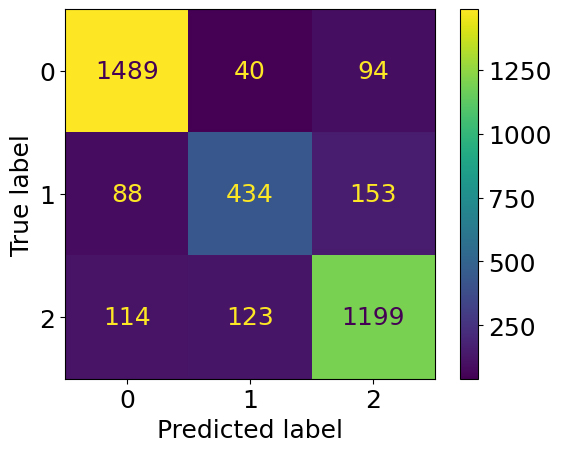
\includegraphics[width=0.65\textwidth]{figure14.jpg}
    \caption{Confusion matrix for K-Nearest Neighbors (KNN) classification}
    \label{fig:figur14}
\end{figure}


\begin{table}[htbp]
  \centering
\caption{Classification report for K-Nearest Neighbors (KNN)}
  \begin{tabular}{|l|l|l|l|l|}
    \hline
                 & Precision & Recall & F1-score & Support \\ \hline
    Group 0.0    & 0.88      & 0.92   & 0.90     & 1623    \\ \hline
    Group 1.0    & 0.73      & 0.64   & 0.68     & 675     \\ \hline
    Group 2.0    & 0.83      & 0.83   & 0.83     & 1436    \\ \hline
    Accuracy     &           &        & 0.84     & 3734    \\ \hline
    Macro avg    & 0.81      & 0.80   & 0.80     & 3734    \\ \hline
    Weighted avg & 0.83      & 0.84   & 0.83     & 3734    \\ \hline
  \end{tabular}
  \label{tab:results}
\end{table}



Due of its accessibility, Decision Tree is an extensively utilised strategy for categorization issues. The central node stands for a certain trait, whereas each leaf node indicates a potential consequence. Decision trees have the benefit of not requiring characteristics to be normalised, which speeds up pre-processing. 



\subsection{Decision tree classifier}

When there is an imbalance in the dataset, overfitting may easily happen with noisy data and provide biased conclusions. When compared to the K-Nearest Neighbour model Table~\ref{tab:updated_results}, the decision tree technique displayed excellent accuracy of 0.87, which is noteworthy.


\begin{table}[htbp]
  \centering
  \caption{DT classification report}
  \begin{tabular}{|l|l|l|l|l|}
    \hline
                 & Precision & Recall & F1-score & Support \\ \hline
    Group 0.0    & 0.92      & 0.92   & 0.92     & 1623    \\ \hline
    Group 1.0    & 0.77      & 0.78   & 0.78     & 675     \\ \hline
    Group 2.0    & 0.87      & 0.87   & 0.87     & 1436    \\ \hline
    Accuracy     &           &        & 0.87     & 3734    \\ \hline
    Macro avg    & 0.85      & 0.86   & 0.85     & 3734    \\ \hline
    Weighted avg & 0.87      & 0.87   & 0.87     & 3734    \\ \hline
  \end{tabular}
  \label{tab:updated_results}
\end{table}


\subsection{Naive Bayes}
A group of decision trees make up Naive Bayes. It votes on the optimal decision tree to use out of a selection of randomly generated decision trees selected from the training data. The Naive Bayes model does not suffer from overfitting problems, which are a problem with other approaches. In contrast to the other models, the Naive Bayes model had a comparatively low accuracy of just 0.57 Table~\ref{tab:updated_results_2}.


\begin{table}[htbp]
  \centering
  \caption{NB classification report}
  \begin{tabular}{|l|l|l|l|l|}
    \hline
                 & Precision & Recall & F1-score & Support \\ \hline
    Group 0.0    & 0.61      & 0.76   & 0.68     & 1623    \\ \hline
    Group 1.0    & 0.26      & 0.05   & 0.08     & 675     \\ \hline
    Group 2.0    & 0.54      & 0.60   & 0.56     & 1436    \\ \hline
    Accuracy     &           &        & 0.57     & 3734    \\ \hline
    Macro avg    & 0.47      & 0.47   & 0.44     & 3734    \\ \hline
    Weighted avg & 0.52      & 0.57   & 0.53     & 3734    \\ \hline
  \end{tabular}
  \label{tab:updated_results_2}
\end{table}

\section{Conclusion}

Except for the Naive Bayes model, all models showed good performance and high accuracy. Accuracy rates for the K-NN and Decision Tree models were 84\% and 87\%, respectively. The accuracy of the Naive Bayes model was just 57\%, which shows space for improvement. A more thorough search for the optimum hyperparameters should be done to optimize these models further. \\
But it's important to remember that stress is ultimately subjective and that different people react to it in various ways. Therefore, the most reliable stress monitoring techniques rely on unique physiological signal fluctuations. ML models based on physiological data are unsuitable for real-world stress monitoring systems because they cannot properly predict the stress of novel, unknown individuals. Only person-specific models are accurate enough for this goal \cite{ravi2021}.  Person-specific models are stiff and expensive to apply in real-world settings because, in contrast to generic models, they must be trained from scratch for each system user. This requires gathering and training a new model for each person utilizing expensive resources in an office scenario \cite{ravi2021}. Additionally, because stress is inherently dynamic, these models will need expensive routine updates to gather and retrain each model to minimize system degeneration brought on by concept drift. \\

Finally, even though the K-NN and Decision Tree models show promise in terms of accuracy, their practical application may provide difficulties. Given individual variances and the dynamic nature of stress, it is critical to strike a balance between model accuracy and the viability of using these models in real-world scenarios.



%%%%%%%%%%%%%%%%%%%%%%%%%%%

\begin{thebibliography}{}
\bibitem{zhang2017}
X. Zhang, Y. Zhao, and B. Guo, "Deep learning-based stress recognition from physiological signals," in \textit{IEEE International Conference on Bioinformatics and Biomedicine (BIBM)}, 2017, pp. 1278-1281.

\bibitem{nkurikiyeyezu}
K. Nkurikiyeyezu, A. Yokokubo, and G. Lopez, "The Influence of Person-Specific Biometrics in Improving Generic Stress Predictive Models," \textit{Wearable Environment and Information Systems Lab, Aoyama Gakuin University}, 5-10-1 Fuchinobe Chuo-ku, Sagamihara-shi, Kanagawa-ken 252-5258, Japan.

\bibitem{cohen2007}
S. Cohen, D. Janicki-Deverts, and G. E. Miller, "Psychological stress and disease," \textit{JAMA}, vol. 298, no. 14, pp. 1685-1687, 2007.

\bibitem{sharma2012}
N. Sharma and T. Gedeon, "Objective measures, sensors and computational techniques for stress recognition and classification: A survey," \textit{Computer Methods and Programs in Biomedicine}, vol. 108, no. 3, pp. 1287-1301, 2012.

\bibitem{healey2005}
J. A. Healey and R. W. Picard, "Detecting stress during real-world driving tasks using physiological sensors," \textit{IEEE Transactions on Intelligent Transportation Systems}, vol. 6, no. 2, pp. 156-166, 2005.

\bibitem{calvo2010}
R. A. Calvo and S. D'Mello, "Affect detection: An interdisciplinary review of models, methods, and their applications," \textit{IEEE Transactions on Affective Computing}, vol. 1, no. 1, pp. 18-37, 2010.

\bibitem{sano2013}
A. Sano and R. W. Picard, "Stress recognition using wearable sensors and mobile phones," in \textit{Humaine Association Conference on Affective Computing and Intelligent Interaction (ACII)}, 2013, pp. 671-676.

\bibitem{ravi2021}
M. S. Ravi, "Stress-detection-in-nurse," 2021. [Online]. Available: \url{https://github.com/CPHSLab/Stress-Detection-in-Nurses}
\end{thebibliography}



\end{document}